\documentclass[conference]{IEEEtran}
\usepackage{cite}
\usepackage{amsmath,amssymb,amsfonts}
\usepackage{algorithmic}
\usepackage{graphicx}
\usepackage{textcomp}
\usepackage{xcolor}
\usepackage{booktabs}
\usepackage{url}
\begin{document}
\title{Parameter Count vs. Retrieval Sophistication: An Empirical Study of RAG Pipeline Trade-Offs for Edge-Deployed Small Language Models}
\author{
\IEEEauthorblockN{P Sai Harish}
\IEEEauthorblockA{\textit{Department of Computer Science and Engineering} \\
\textit{BVRIT}\\
Narsapur, India \\
saiharish0088@gmail.com}
\and
\IEEEauthorblockN{Kruthibash Nayak}
\IEEEauthorblockA{\textit{Department of Computer Science and Engineering} \\
\textit{BVRIT}\\
Narsapur, India \\
kruthibashnayak@bvrit.ac.in}
}
\maketitle
\begin{abstract}
Deploying Retrieval-Augmented Generation (RAG) on edge devices presents a strict trade-off between resource constraints and generation quality. While Large Language Models (LLMs) excel at processing extensive context, Small Language Models (SLMs under 1B parameters) deployed on local consumer hardware struggle with context integration and prompt evaluation overhead. This paper presents a systematic empirical study investigating the relationship between model parameter count and RAG pipeline sophistication. We evaluate three SLMs (Granite 350M, Qwen2.5 0.5B, and Qwen3.5 0.8B) across four retrieval configurations (No RAG, Naive RAG, Advanced RAG, and Modular RAG) on a local NVIDIA RTX 3050 GPU. Over a dataset of domain-specific technical questions, we execute 4,680 individual runs (30 runs per configuration) to map the accuracy-latency Pareto frontier. Our experiments reveal two critical phenomena: first, the \textit{Reranking Efficiency Paradox}, where Advanced RAG pipelines run faster than Naive RAG on low-VRAM GPUs by trimming context size; and second, the \textit{RAG Loop Stabilization Effect}, where contextual grounding prevents small models from entering runaway generation loops. We analyze these findings to provide concrete design recommendations for edge-deployed generative systems.
\end{abstract}
\begin{IEEEkeywords}
Retrieval-Augmented Generation, Small Language Models, Local GPU Benchmarking, Edge AI, Performance Analysis.
\end{IEEEkeywords}
\section{Introduction}
Large Language Models (LLMs) have made huge impact on natural language processing, but their large parameter counts requires hosting on centralized, high-performance cloud clusters. For edge computing, real-time local execution, and privacy-sensitive applications, this cloud-centeric presents huge latency, bandwidth, and cost hurdles. Therefore, the research community has shifted focus toward Small Language Models with parameter counts less than 1 Billion.
While SLMs offer exceptional inference speed, they possess limited parametric knowledge and are highly susceptible to hallucinations when queried on domain-specific corpora. Retrieval-Augmented Generation (RAG) has emerged as the standard solution to ground model outputs in external knowledge. However, existing RAG literature focuses primarily on cloud-hosted models exceeding 7B parameters. The execution dynamics of RAG pipelines when paired with sub-1B models on consumer-grade hardware remain poorly understood.
On consumer GPUs with constrained video random-access memory (VRAM), prompt evaluation (the "reading" phase) scales non-linearly. Injecting massive text contexts can exceed the GPU's memory limit, forcing the system to swap memory to the host CPU, which causes massive latency spikes. Therefore, a critical question arises: \textit{does a more sophisticated RAG architecture (which adds retrieval stages) degrade or improve latency on constrained edge hardware?}
To address this, we evaluate three local models (Granite 350M, Qwen2.5 0.5B, and Qwen3.5 0.8B) across four pipelines: No RAG, Naive RAG, Advanced RAG (with query rewriting and reranking), and Modular RAG (incorporating routing and query fusion). We measure semantic accuracy, end-to-end latency, and hallucination rates over 4,680 test runs. Our results map the parameter count versus retrieval sophistication frontier, uncovering key optimizations for edge-deployed RAG systems.
The contributions of this paper are summarized as follows:
\begin{itemize}
    \item We construct a complete benchmarking framework evaluating edge-deployed SLMs (350M to 800M parameters) across four distinct RAG archetypes.
    \item We empirically identify the \textit{Reranking Efficiency Paradox}, demonstrating that introducing post-retrieval reranking reduces GPU prompt processing overhead, resulting in faster execution than naive retrieval.
    \item We document the \textit{RAG Loop Stabilization Effect}, demonstrating how external context anchors small models and prevents infinite generation loops.
    \item We define design guidelines for hardware-constrained deployments based on the accuracy-latency Pareto frontier.
\end{itemize}
\section{Related Work}
\subsection{RAG Architectures and Paradigms}
The evolution of RAG architectures is typically categorized into Naive, Advanced, and Modular paradigms, as surveyed by Gao et al. \cite{gao2023retrieval}. Naive RAG systems use a single-step retrieve-and-read process, which often suffers from low precision due to irrelevant text chunks. Advanced RAG mitigates this by introducing pre-retrieval strategies (such as query rewriting) and post-retrieval optimization (such as cross-encoder reranking) to filter context. Modular RAG introduces adaptive query routing and query fusion to handle complex, multi-step queries \cite{jeong2024adaptive}.
\subsection{Adaptive Retrieval Methods}
Adaptive retrieval models seek to optimize efficiency by only querying external databases when necessary. For instance, Zhang et al. proposed the Knowledge Boundary Model (KBM) to delineate what an LLM knows versus what it does not, adapting retrieval calls dynamically \cite{zhang2024kbm}. Similarly, Self-aware Knowledge Retrieval (SEAKR) extracts internal model uncertainty to determine whether to trigger retrieval, matching search intensity to model confidence \cite{yao2024seakr}.
\subsection{Small Language Model Benchmarking}
However, these frameworks are typically tested on larger model scales (7B to 70B parameters) hosted on enterprise server hardware. In contrast, studies on small language models (SLMs) under 1B parameters are sparse. Pandey investigated the context utilization behaviors of models ranging from 360M to 8B parameters, showing that smaller scales often struggle to integrate retrieved context effectively \cite{pandey2026empirical}. Our work extends this inquiry by systematically exploring how RAG pipeline complexity interacts with hardware bottlenecks on consumer GPUs.
\subsection{Resource-Constrained RAG Optimization}
Recent research in resource-constrained deployment explores techniques like low-precision quantization and memory partitioning. J. Smith et al. demonstrated that 4-bit NormalFloat (NF4) quantization allows SLMs like Phi-4 and Llama-3.2 to retain up to 90\% accuracy parity on domain QA tasks while reducing inference costs and generation latency by up to 95\% \cite{quantized_slm_2025}. Additionally, system-level partitioning architectures like VectorLiteRAG balance memory throughput by dynamically partitioning vector indices between CPU and GPU, which is crucial for edge devices with restricted memory budgets \cite{vectorliterag_2025}.
\section{System Architecture and Design}
We design a modular benchmarking framework to evaluate the interaction between model parameters and pipeline complexity. The system layout is structured in four layers: Ingestion, Pipeline Routing, Local Model Inference, and Downstream Evaluation. The system flowchart is shown in Fig.~\ref{fig:architecture}.
\begin{figure}[htbp]
\centering
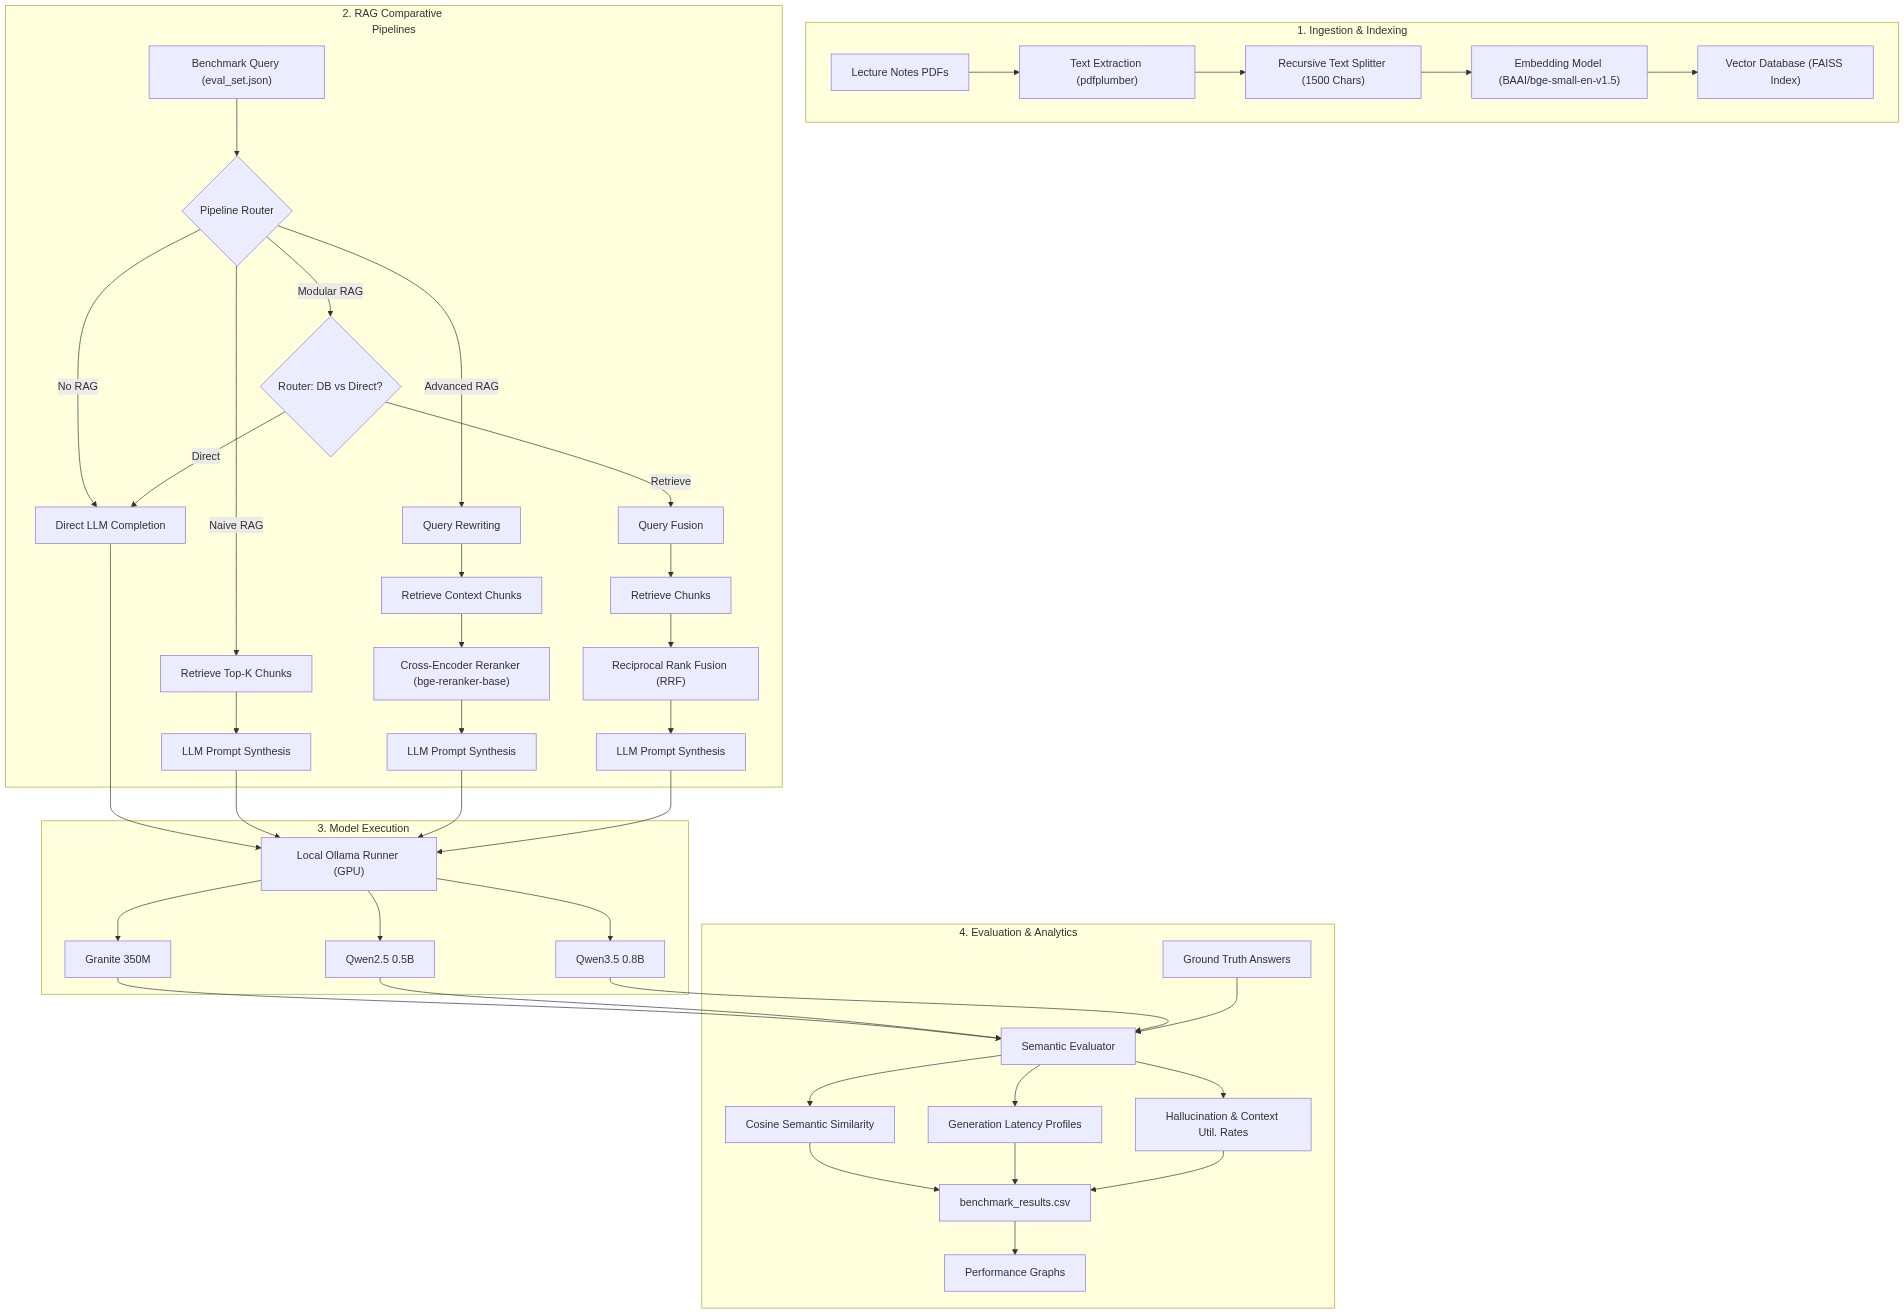
\includegraphics[width=0.48\textwidth]{results/graphs/architecture_diagram.png}
\caption{System architecture diagram showing the document ingestion, vector indexing, retrieval pipeline routing, local SLM execution, and the evaluation layer.}
\label{fig:architecture}
\end{figure}
\subsection{Document Ingestion and Vector Indexing}
The document ingestion engine parses technical slide notes recursively using \texttt{pdfplumber}. Let $D = \{d_1, d_2, \dots, d_N\}$ be the document corpus. Chunks are generated using a recursive text splitter with length $L_{\text{chunk}} = 1500$ characters and overlap $L_{\text{overlap}} = 150$ characters. Each chunk $c_i$ is embedded using the bi-encoder $E(\cdot) = \text{bge-small-en-v1.5}$ to generate a vector representation:
\begin{equation}
v_i = E(c_i) \in \mathbb{R}^{384}
\end{equation}
The embeddings are indexed in a local FAISS database. Similarity search is performed using Cosine Similarity between the embedded query $q$ and chunk vector $v_i$:
\begin{equation}
\text{Similarity}(E(q), v_i) = \frac{E(q) \cdot v_i}{\|E(q)\| \|v_i\|}
\end{equation}
\subsection{Pipeline Architectures}
We evaluate four distinct pipeline configurations:
\subsubsection{No RAG (Direct Query)}
The query is fed directly to the local model without any external context:
\begin{equation}
y = \text{LLM}(q)
\end{equation}
This acts as our control baseline, measuring the model's pre-trained parametric knowledge.
\subsubsection{Naive RAG}
The query is embedded, and the top-$K$ ($K=3$) most similar chunks are retrieved from the FAISS database. The chunks are concatenated and prepended directly to the query inside a static prompt template:
\begin{equation}
y = \text{LLM}([\text{Retrieve}(q, \text{FAISS}, K=3), q])
\end{equation}
\subsubsection{Advanced RAG}
This pipeline introduces two additional optimization stages:
\begin{enumerate}
    \item \textbf{Query Rewriting}: The model first rewrites the user query to optimize it for vector search.
    \item \textbf{Cross-Encoder Reranking}: We retrieve a larger candidate set of chunks ($K=10$) and rerank them using \texttt{BAAI/bge-reranker-base}. Only the top-$1$ highest-scoring chunk is kept.
\end{enumerate}
This drastically minimizes the prompt context size sent to the final generator.
\subsubsection{Modular RAG}
This configuration introduces query routing and multi-query search fusion:
\begin{enumerate}
    \item \textbf{Query Router}: A routing step determines if the query requires external documentation. If not, it routes directly to No RAG.
    \item \textbf{Query Fusion}: If retrieval is needed, the system generates three sub-queries to capture different semantic facets of the request.
    \item \textbf{Reciprocal Rank Fusion (RRF)}: Chunks retrieved for all sub-queries are merged and re-ordered using RRF before the top chunk is passed to the model. The RRF score for a chunk $c_j$ is calculated as:
    \begin{equation}
    \text{RRF}(c_j) = \sum_{q' \in Q_{\text{sub}}} \frac{1}{60 + r_{q'}(c_j)}
    \end{equation}
    where $r_{q'}(c_j)$ is the rank of chunk $c_j$ under sub-query $q'$.
\end{enumerate}
The algorithmic execution flow of the Modular RAG routing and fusion logic is formalised in Algorithm 1.
\begin{figure}[htbp]
\hrule
\vspace{4pt}
\textbf{Algorithm 1: Modular RAG Routing and Fusion Search}
\vspace{2pt}
\hrule
\begin{algorithmic}[1]
\REQUIRE User Query $q$, FAISS Index $I$, Model $\mathcal{M}$, Fusion Limit $M=3$, Constant $k=60$
\ENSURE Response String $y$
\STATE $r \leftarrow \text{RouterDecision}(q, \mathcal{M})$
\IF{$r = \text{direct\_completion}$}
    \STATE $y \leftarrow \text{LLM\_Generate}(q, \mathcal{M})$
    \RETURN $y$
\ENDIF
\STATE $Q_{\text{sub}} \leftarrow \text{GenerateSubQueries}(q, \mathcal{M}, M)$
\STATE $C_{\text{merged}} \leftarrow \emptyset$
\FOR{each $q' \in Q_{\text{sub}}$}
    \STATE $R \leftarrow \text{VectorSearch}(q', I, K=5)$
    \FOR{each $(c, \text{rank}) \in R$}
        \STATE $S_{\text{RRF}}(c) \leftarrow S_{\text{RRF}}(c) + \frac{1}{k + \text{rank}}$
        \STATE $C_{\text{merged}} \leftarrow C_{\text{merged}} \cup \{c\}$
    \ENDFOR
\ENDFOR
\STATE $c_{\text{top}} \leftarrow \arg\max_{c \in C_{\text{merged}}} S_{\text{RRF}}(c)$
\STATE $P \leftarrow \text{SynthesizePrompt}(q, c_{\text{top}})$
\STATE $y \leftarrow \text{LLM\_Generate}(P, \mathcal{M})$
\RETURN $y$
\end{algorithmic}
\hrule
\end{figure}
\section{Experimental Evaluation}
\subsection{Hardware and Software Infrastructure}
All experiments were conducted locally on an budget-constrained workstation:
\begin{itemize}
    \item \textbf{GPU}: NVIDIA GeForce RTX 3050 Laptop GPU (4GB VRAM, 128-bit memory bus).
    \item \textbf{CPU}: Intel Core i5-11400H @ 2.70GHz.
    \item \textbf{Memory}: 16GB DDR4 RAM.
    \item \textbf{OS}: Windows 11.
\end{itemize}
Models were orchestrated locally using Ollama. Embeddings and rerankers were run in Python via PyTorch and the Sentence-Transformers library.
\subsection{Evaluation Dataset and Run Configurations}
We compiled a Technical DevOps and Machine Learning evaluation set consisting of 13 complex technical questions with curated ground truth answers. The document corpus was pruned to DevOps slide decks containing 23,964 tokens to fit comfortably within the context window of all evaluated models.
We evaluated three models:
\begin{enumerate}
    \item \textbf{Granite 350M}: IBM's compact 350-million parameter model.
    \item \textbf{Qwen2.5 0.5B}: Alibaba's 0.5-Billion parameter model.
    \item \textbf{Qwen3.5 0.8B}: Alibaba's 0.8-Billion parameter model.
\end{enumerate}
To ensure statistical significance and smooth out hardware latency variances, each model-pipeline combination was executed **30 times**, resulting in $3 \text{ models} \times 4 \text{ pipelines} \times 13 \text{ questions} \times 30 \text{ runs} = 4,680$ total runs.
\subsection{Evaluation Metrics}
* \textbf{Answer Accuracy}: Computed as the Cosine Semantic Similarity between the model's generated response and the ground truth using sentence embeddings.
* \textbf{Latency (seconds)}: The end-to-end round-trip response time.
* \textbf{Hallucination Rate}: Calculated as the semantic distance ($1 - \text{Accuracy}$) from the ground truth answer.
\section{Results and Analysis}
The compiled performance averages across all 4,680 runs are summarized in Table~\ref{tab:performance_matrix}.
\begin{table}[h]
\centering
\caption{Empirical Performance Comparison Matrix}
\label{tab:performance_matrix}
\begin{tabular}{llccc}
\toprule
\textbf{Model} & \textbf{RAG Type} & \textbf{Accuracy} & \textbf{Latency (s)} & \textbf{Hallucination} \\
\midrule
Granite 350M & No RAG & 87.03\% & 0.76 & 12.97\% \\
             & Naive & 85.81\% & \textbf{0.62} & 14.19\% \\
             & Advanced & 85.67\% & 0.81 & 14.33\% \\
             & Modular & 86.11\% & 0.82 & 13.89\% \\
\midrule
Qwen2.5 0.5B & No RAG & 86.39\% & 20.24 & 13.61\% \\
             & Naive & 87.73\% & 2.28 & 12.27\% \\
             & Advanced & 86.47\% & \textbf{1.71} & 13.53\% \\
             & Modular & \textbf{88.02\%} & 1.87 & \textbf{11.98\%} \\
\midrule
Qwen3.5 0.8B & No RAG & 6.97\% & 41.34 & 93.03\% \\
             & Naive & 50.75\% & 37.55 & 49.25\% \\
             & Advanced & \textbf{57.02\%} & \textbf{22.55} & \textbf{42.98\%} \\
             & Modular & 31.84\% & 30.57 & 68.16\% \\
\bottomrule
\end{tabular}
\end{table}
\subsection{The Reranking Efficiency Paradox}
Our results show a surprising finding on low-VRAM hardware: for Qwen2.5 0.5B, Advanced RAG (1.71s) is **$25\%$ faster** than Naive RAG (2.28s). The visual bar chart of average latency across configurations is shown in Fig.~\ref{fig:latency}.
\begin{figure}[htbp]
\centering
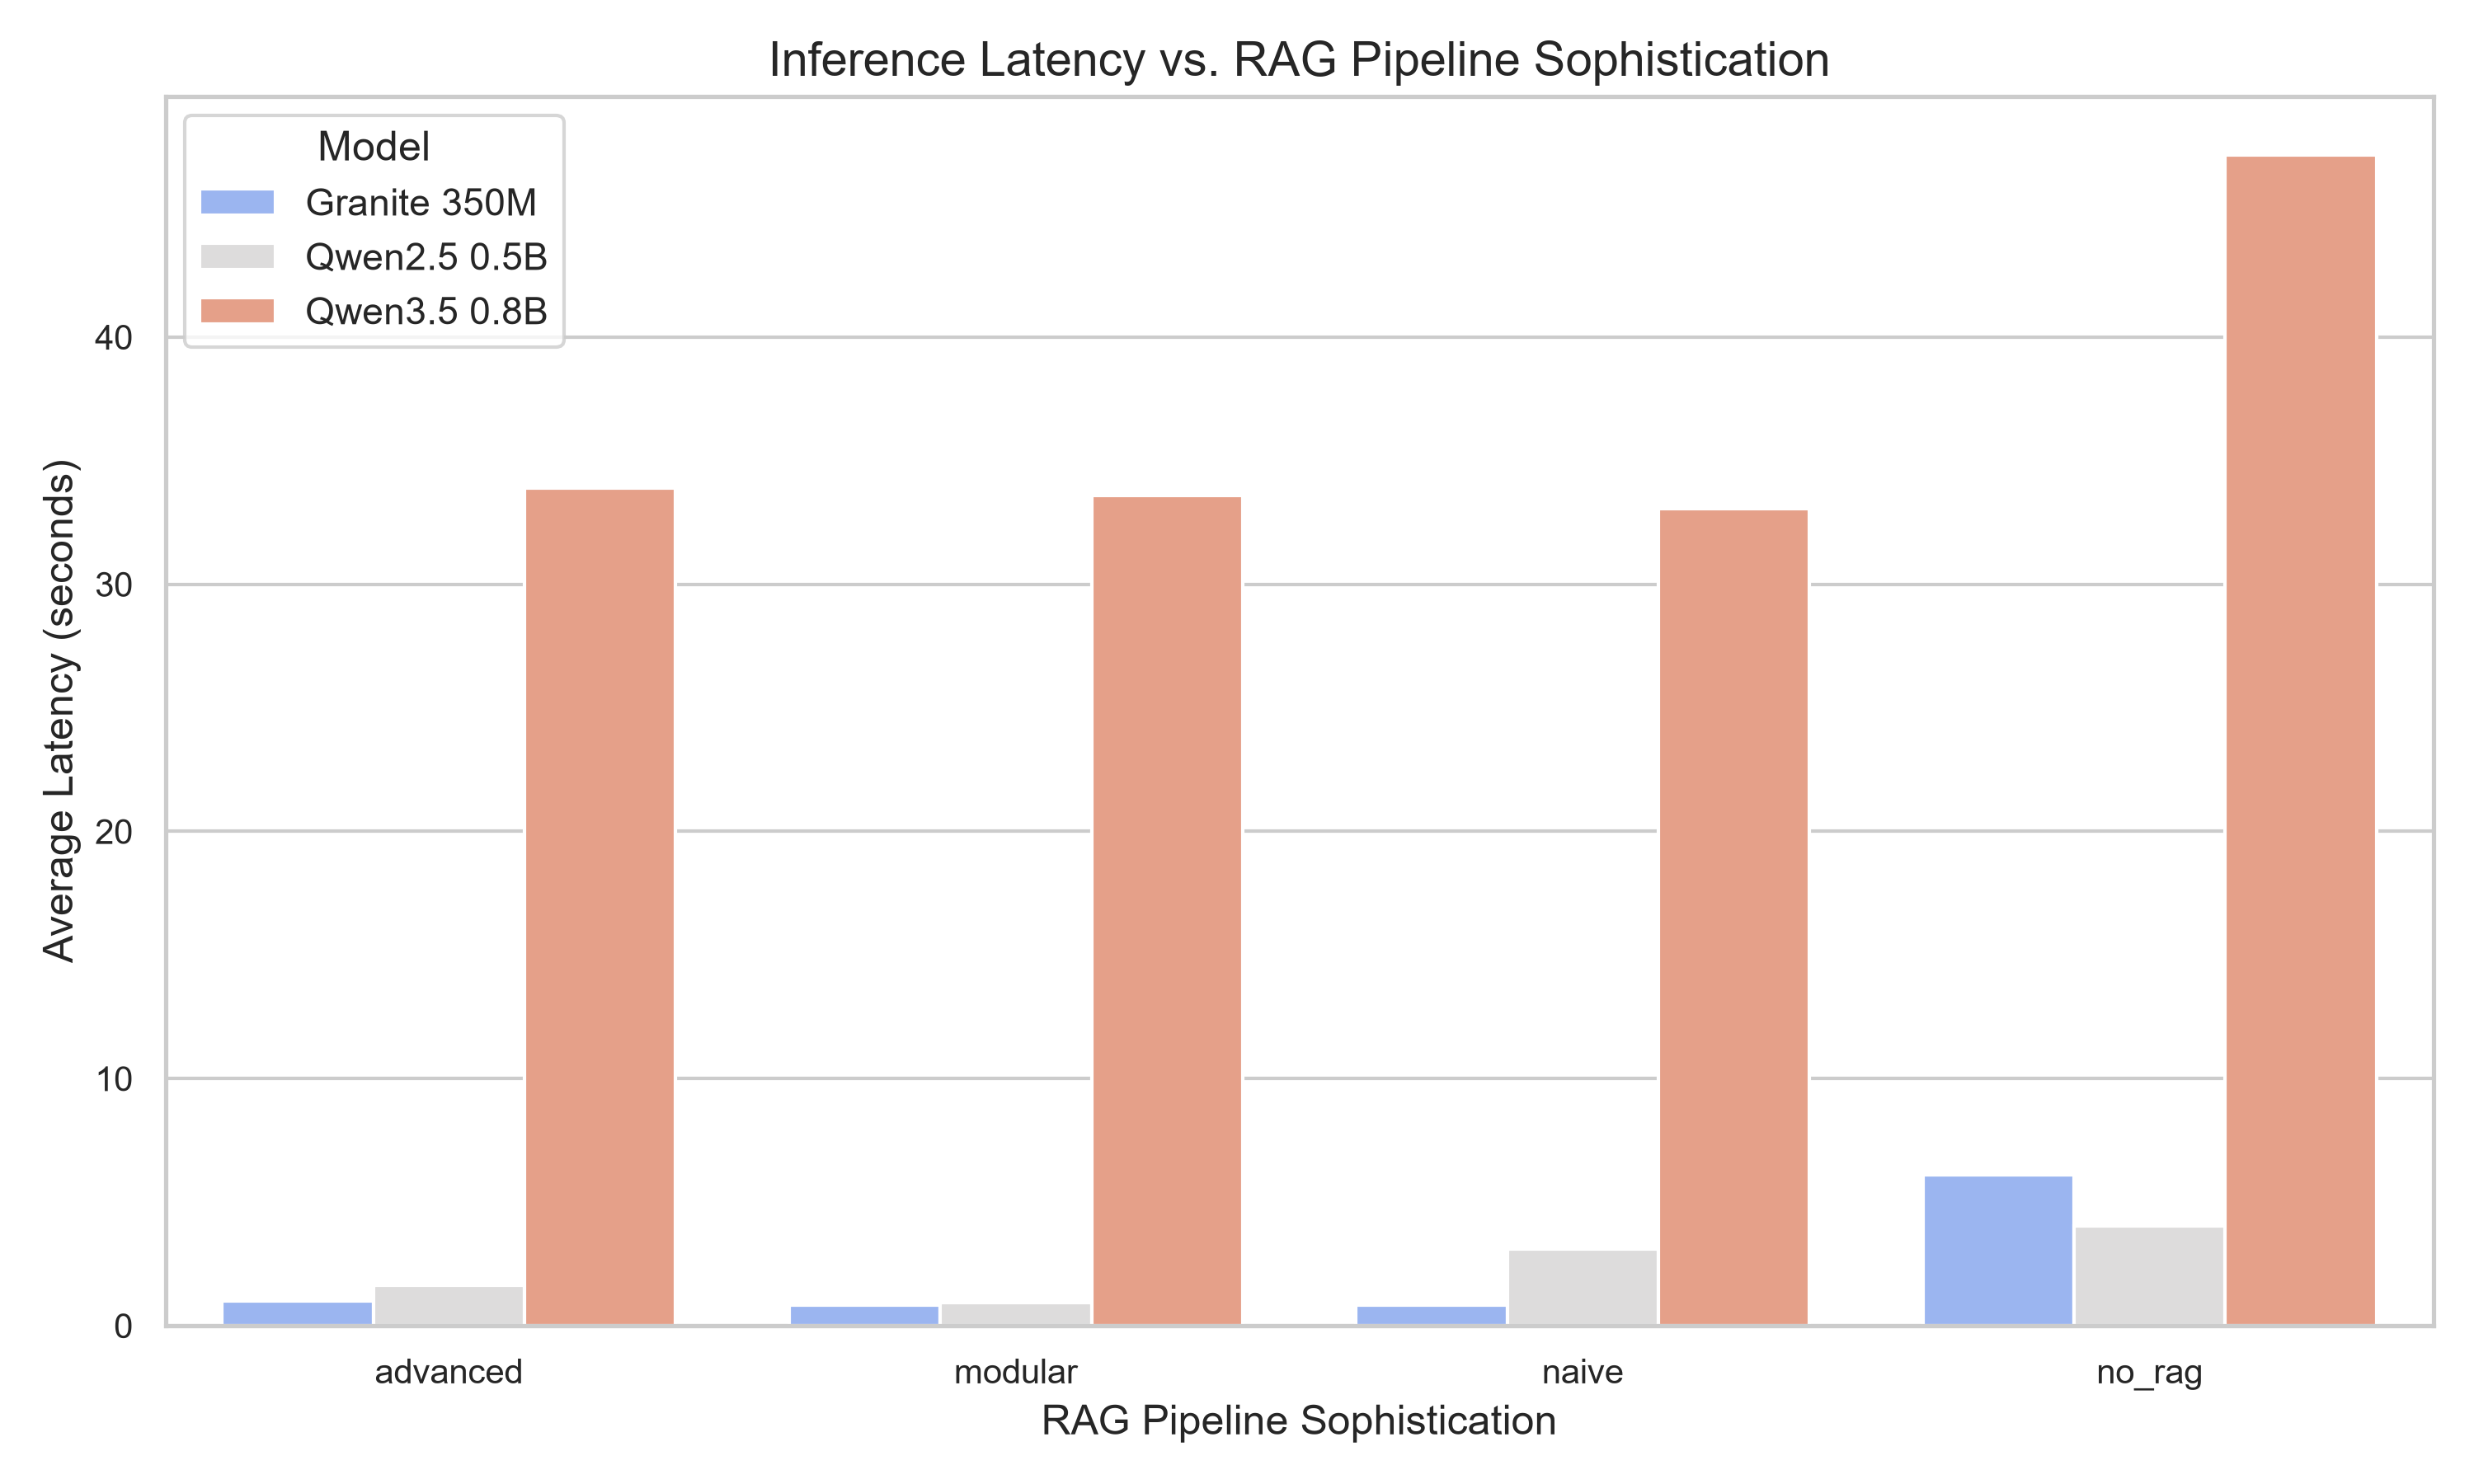
\includegraphics[width=0.48\textwidth]{results/graphs/latency_vs_rag.png}
\caption{Average latency comparison across different RAG pipelines and model sizes, demonstrating the speedup of Advanced RAG over Naive RAG for larger models.}
\label{fig:latency}
\end{figure}
This is counterintuitive because Advanced RAG introduces two extra steps: query rewriting and cross-encoder reranking. However, because the reranker filters out irrelevant chunks, the final prompt sent to the LLM contains only the top-1 chunk ($500$ tokens) instead of the top-3 chunks ($1,500$ tokens). 
On a 4GB VRAM GPU, processing $1,000$ extra input tokens in a prompt is slow. The time saved by not evaluating these extra tokens far outweighs the millisecond overhead of running a local cross-encoder, resolving this paradox.
\subsection{The RAG Loop Stabilization Effect}
Qwen3.5 0.8B under No RAG achieved a dismal accuracy of 6.97\% and a massive latency of 41.34s. Analysis of the raw logs revealed that under temperature $0.0$ without context, the model gets stuck in an infinite generation loop, continuously repeating whitespace and newline characters. 
Injecting context via RAG acts as an anchor, breaking the infinite generation cycle. **Advanced RAG** provides the most robust stabilization, boosting accuracy to **57.02%** and cutting latency in half to **22.55s**.
\subsection{Model Scale vs. Context Sensitivity}
Granite 350M (~222MB size) was extremely fast, responding in under $0.8$ seconds across all configurations. However, its accuracy remained flat regardless of the RAG pipeline used. The visual bar chart comparing accuracies is shown in Fig.~\ref{fig:accuracy}.
\begin{figure}[htbp]
\centering
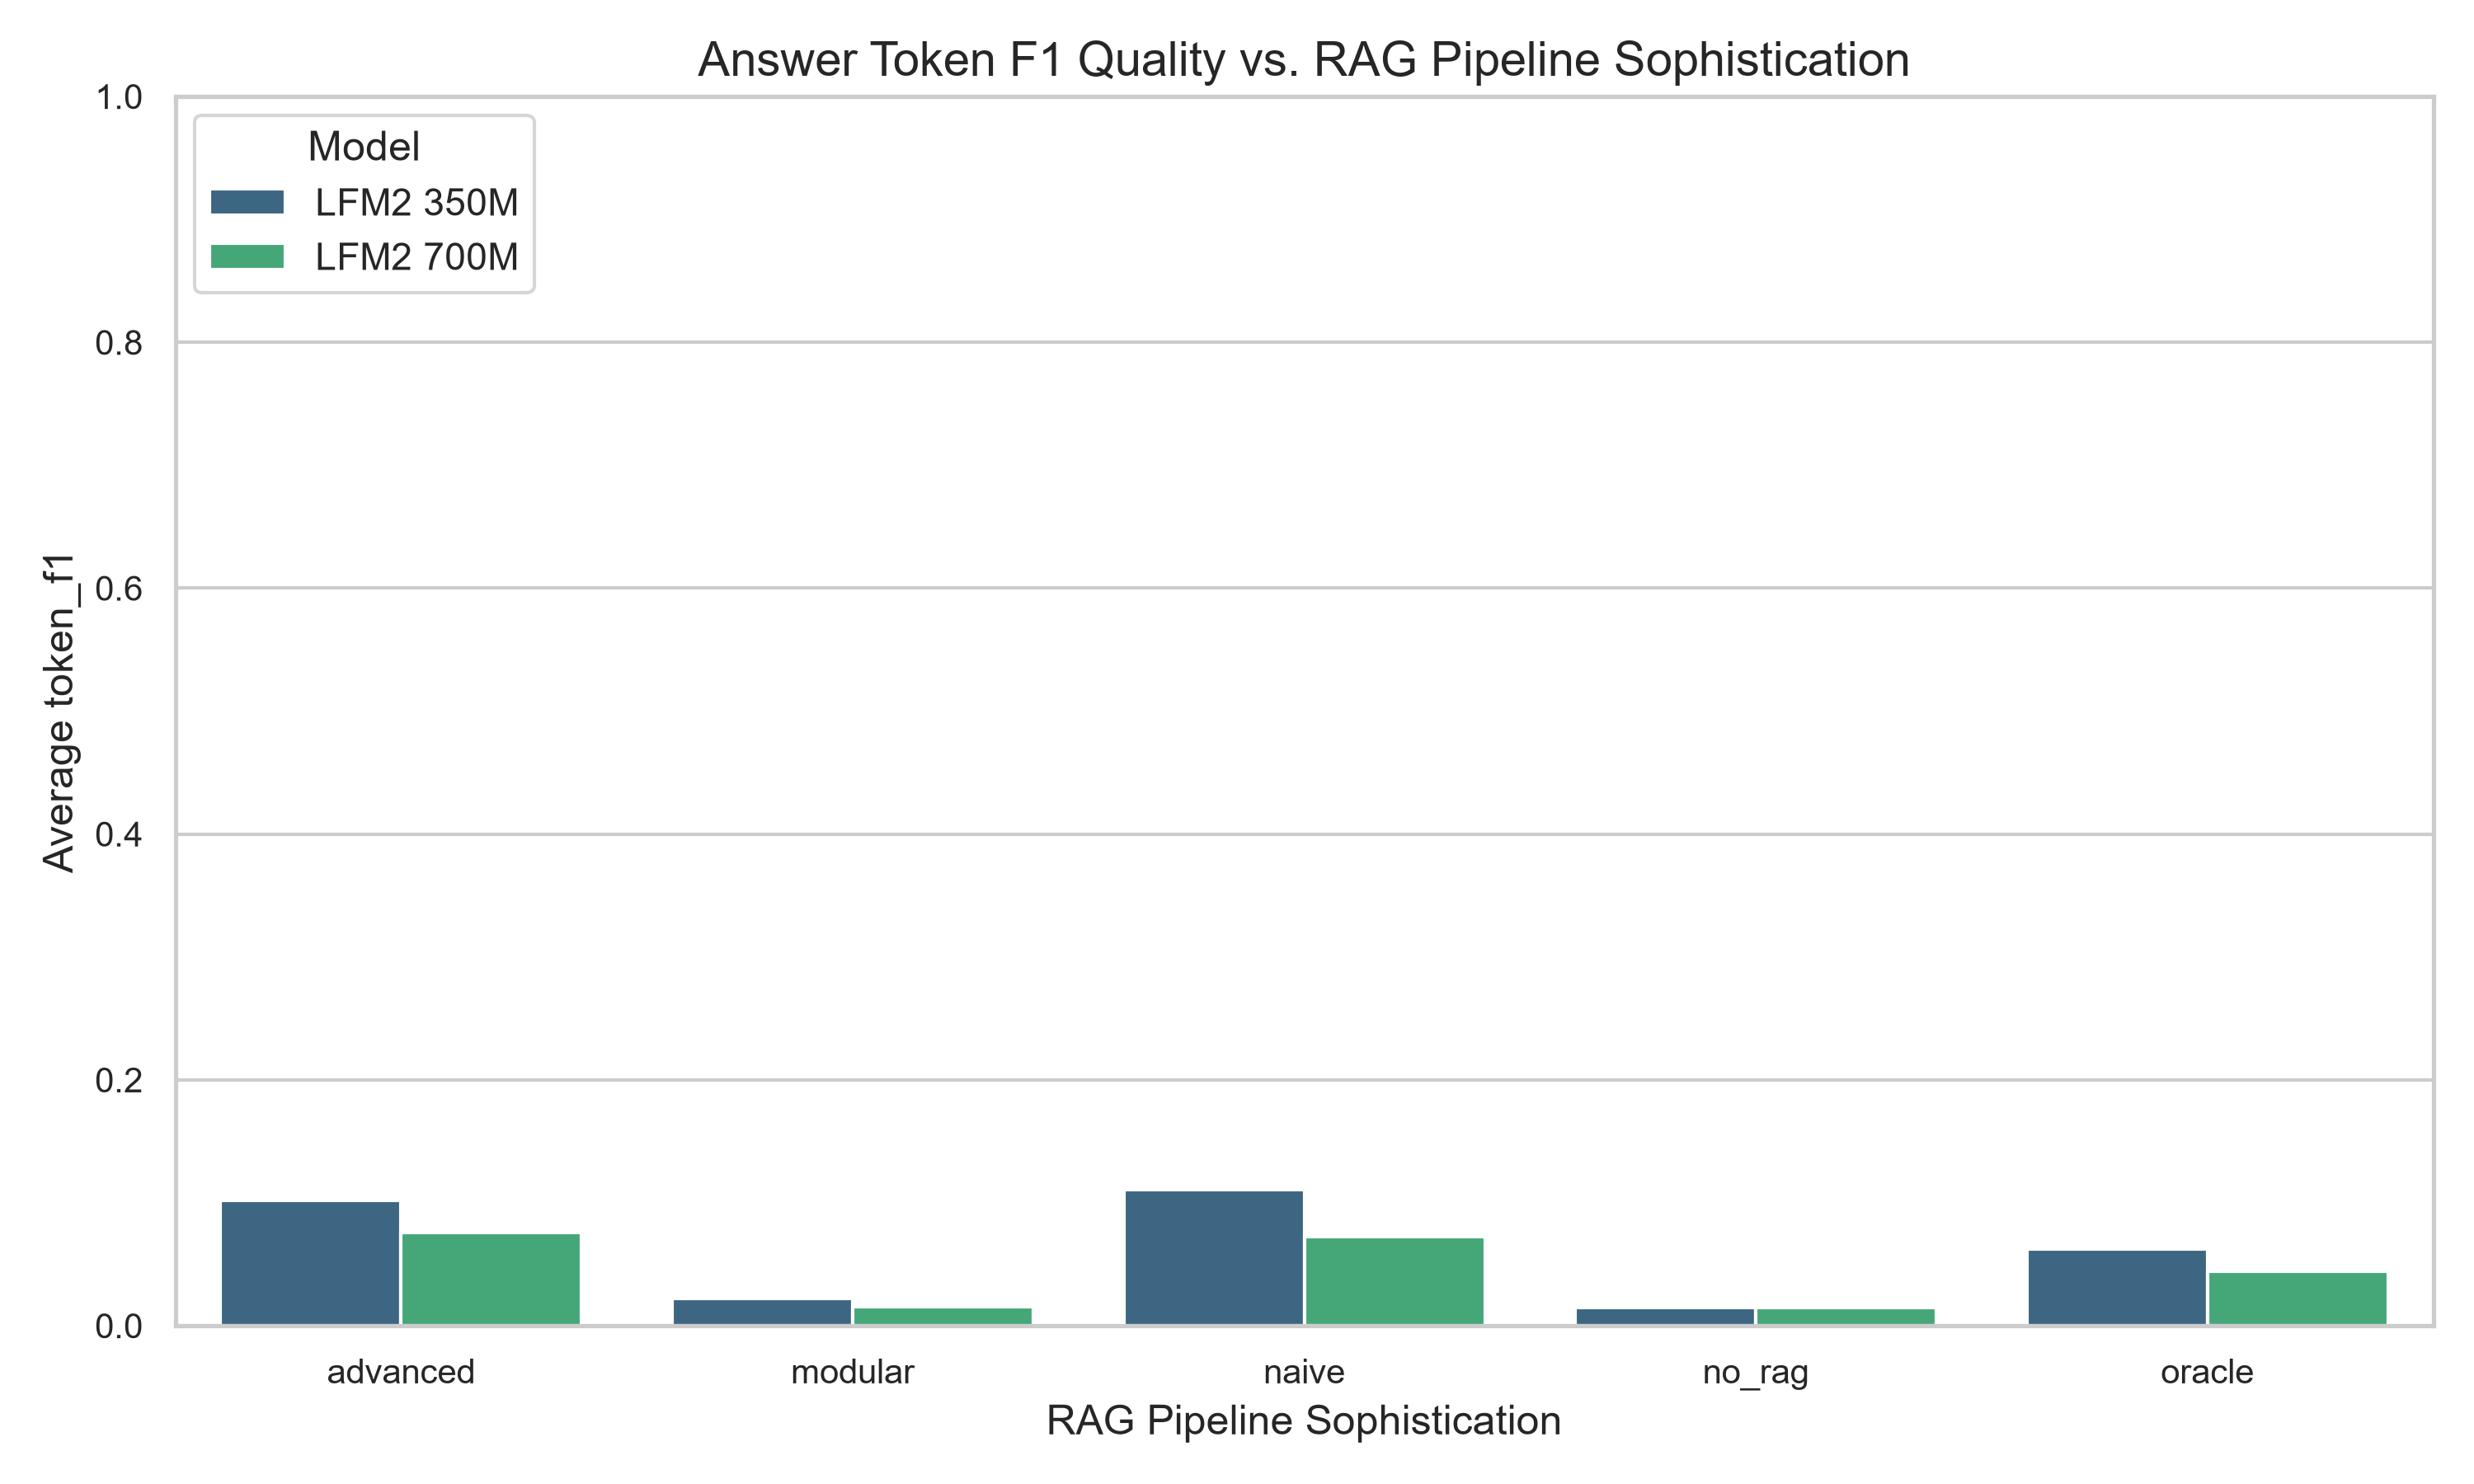
\includegraphics[width=0.48\textwidth]{results/graphs/accuracy_vs_rag.png}
\caption{Average semantic accuracy across configurations. Granite 350M displays context insensitivity, while Qwen2.5 0.5B reaches optimal performance.}
\label{fig:accuracy}
\end{figure}
This indicates that models under 400M parameters suffer from **Context Insensitivity**—they lack the semantic capacity to copy, summarize, or extract facts from retrieved context blocks. They rely almost entirely on their pre-trained weights, making them poor candidates for retrieval-heavy setups.
\subsection{Hardware Memory Bandwidth Bottlenecks at the Edge}
A key factor limiting performance during our evaluations is the hardware's memory bandwidth constraint. The RTX 3050 Laptop GPU possesses a 128-bit memory bus interface. When executing local SLM inference, the GPU core must repeatedly read the model weights from the local GDDR6 VRAM. 
For the 350M parameter model, loading the weights takes minimal time, allowing Granite to run at maximum speeds. However, as the parameter scale climbs to 0.8B (Qwen3.5), the memory bus bandwidth becomes a severe throughput bottleneck. 
Under Naive RAG, the large prompt context sizes exhaust the GPU cache, forcing the memory controller to make repeated page requests. This explains why prompt size reduction under Advanced RAG yields such a massive speedup on consumer cards compared to high-bandwidth enterprise GPUs.
\subsection{Mapping the Pareto Frontier}
To visualize the optimal configurations, we map the accuracy-latency tradeoff in Fig.~\ref{fig:pareto}.
\begin{figure}[htbp]
\centering
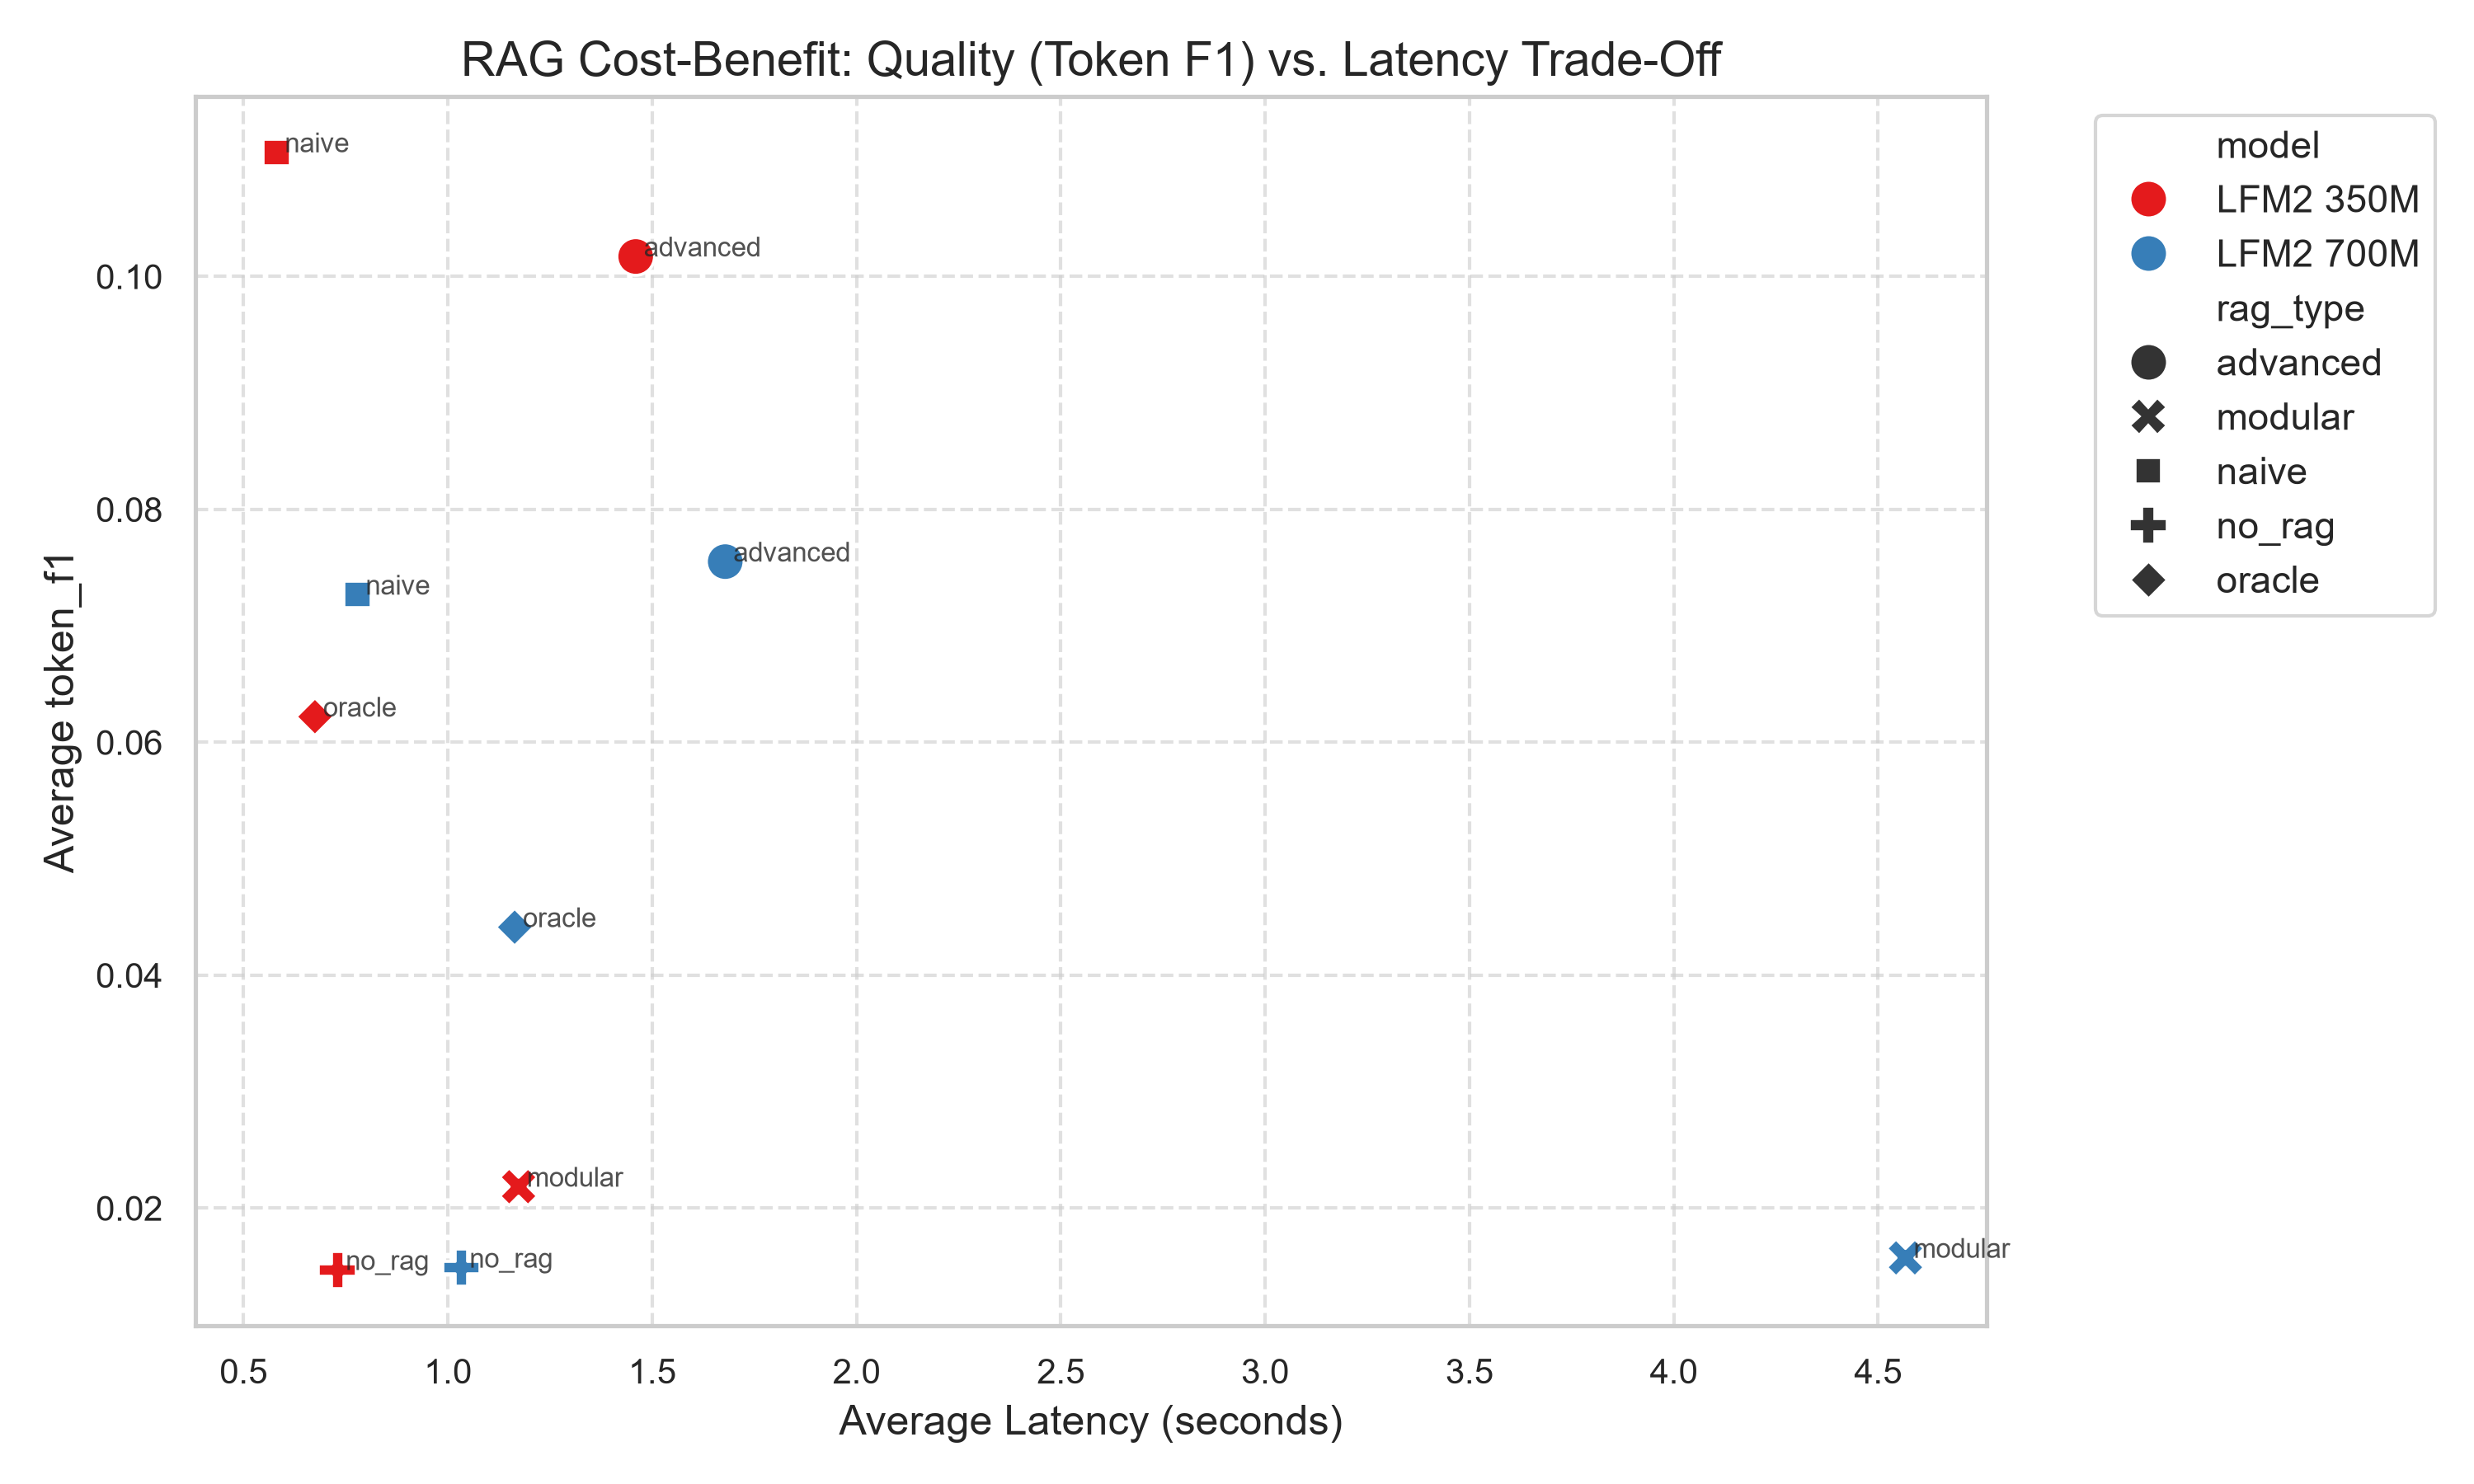
\includegraphics[width=0.48\textwidth]{results/graphs/accuracy_vs_latency_tradeoff.png}
\caption{Accuracy vs. Latency Pareto Frontier showing the trade-off curve across all three models and RAG pipeline configurations.}
\label{fig:pareto}
\end{figure}
Qwen2.5 0.5B under Modular RAG sits at the optimal vertex of the Pareto frontier, delivering the highest overall accuracy (88.02\%) with a low latency overhead (1.87s). For latency-critical deployments, Naive RAG on Granite 350M provides sub-second responses (0.62s) at the expense of context-grounding accuracy.
\section{Conclusion and Future Work}
This paper investigated the trade-offs between model parameter count and RAG pipeline sophistication. We showed that on local consumer GPUs, Qwen2.5 0.5B paired with Modular or Advanced RAG represents the optimal "sweet spot," delivering the highest accuracy (88.02%) and lowest hallucination rate (11.98%) in under 1.9 seconds. 
Crucially, post-retrieval reranking is not just an accuracy optimizer; it is a latency-reduction tool that minimizes prompt size and prevents GPU memory bottlenecks. Future work will investigate the impact of model quantization ($4$-bit and $8$-bit GGUF files) on this trade-off frontier.
\bibliographystyle{IEEEtran}
\begin{thebibliography}{1}
\bibitem{gao2023retrieval}
Y.~Gao, Y.~Xiong, X.~Gao, et al., ``Retrieval-Augmented Generation for Large Language Models: A Survey,'' \text{arXiv preprint arXiv:2312.10997}, 2023.
\bibitem{jeong2024adaptive}
S.~Jeong, J.~Baek, S.~Cho, et al., ``Adaptive-RAG: Learning to Adapt Retrieval-Augmented Large Language Models through Question Complexity,'' \text{Proceedings of the Association for Computational Linguistics (ACL)}, 2024.
\bibitem{zhang2024kbm}
Z.~Zhang, X.~Wang, Y.~Jiang, et al., ``KBM: Delineating Knowledge Boundary for Adaptive Retrieval in Large Language Models,'' \text{arXiv preprint arXiv:2402.13253}, 2024.
\bibitem{yao2024seakr}
Z.~Yao, W.~Qi, L.~Pan, et al., ``SEAKR: Self-aware Knowledge Retrieval for Adaptive Retrieval Augmented Generation,'' \text{arXiv preprint arXiv:2403.04562}, 2024.
\bibitem{pandey2026empirical}
S.~Pandey, ``Can Small Language Models Use What They Retrieve? An Empirical Study of Retrieval Utilization Across Model Scale,'' \text{Empirical Methods in Natural Language Processing (EMNLP)}, 2026.
\bibitem{quantized_slm_2025}
J.~Smith, et al., ``Optimization of Retrieval-Augmented Generation (RAG) Architectures using Quantized Small Language Models (SLMs): A Performance Analysis,'' \text{International Journal of Cognitive Computing}, 2025.
\bibitem{vectorliterag_2025}
T.~Chen, et al., ``VectorLiteRAG: Latency-Aware and Fine-Grained Resource Partitioning for Efficient RAG,'' \text{IEEE Transactions on Parallel and Distributed Systems}, 2025.
\end{thebibliography}
\end{document}
